
\documentclass{article}
\usepackage{amsmath,cite,url}
\usepackage{graphicx}
\usepackage{color}

\newcommand{\ipt}{IPT}

\newcommand{\ml}[1]{\textcolor{blue}{ML : #1}}

% Title.
% ------
\title{Spontaneous Similarity Judgments of Musical Tones played with various Playing Techniques}

\author{Christian El-Hajj, Mathias Rossignol, Grégoire Lafay, Mathieu Lagrange}

\sloppy % please retain sloppy command for improved formatting

\begin{document}
%
\maketitle
%
\begin{abstract}

Musical timbre is a multi-faceted notion that have been extensively studied, mostly focusing on its spectral aspect. By studying the spontaneous judgments of similarity between several instruments played with a diverse set of playing techniques, we aim in this paper at better understanding the influence of the change of the playing technique on the perception of timbre.

A first experiment is conducted by music experts to identify which couple of instrument and playing technique in a given dataset is worth comparing to other couples of instrument / playing technique. In a second experiment, spontaneous similarity judgments among the retained couples are collected using a canonic free sorting task experiment design.


To further study the outcomes of this experiment, we assume a two-step computational model of human perception, where the acoustic signal is fed to a statically designed processing unit that accounts for frequency and temporal modulations. The resulting features are then projected using a supervised technique which considers as input the perceptual similarity judgments gathered in the second experiment. Numerical experiments show that the induced perceptual space is able to approximate perceptual data with satisfying accuracy.

\end{abstract}
%
\section{Introduction}\label{sec:introduction}

Musical timbre is an interesting notion to study as it is perceptively defined \cite{grey1977multidimensional}. Thus, by studying musical timbre, one study many facets of the human auditory system which responds to a diverse set of physical stimuli. However this diversity can be more easily more controlled than other stimuli such as speech or environmental sounds.

The focus of this paper is to study the influence of the playing technique on the perception of timbre.

A popular view of the kind of stimuli we consider is that they can be described by a spread of energy that evolve through time and across frequency. By following this trend, most researchers translate the exclusion definition of timbre \cite{marozeau2003dependency} into a more specified definition. The exclusion definition states that timbre is "the fourth component of sound quality, the first three being pitch, loudness and duration". In an attempt to specify more this notion of timbre, we will loosely consider in this paper that musical timbre is the influence on the human auditory system of the distribution of intensity across the time / frequency plane.

A great deal of litterature focuses on the instantaneous spectrum \cite{grey1978perceptual}. Other studies also demonstrated the importance of the onset in the recognition of some musical instruments. All those studies generally assume a rather short term model where the waveform is observed in a range that do not exceed 100 ms, a common porcessing scenario that is very commonly used in computational recognition models of timbre \cite{tzanetakis2002musical}.

Agus \& al effectively showed that a great deal of instrument recognition can be achieved with very little listening time \cite{agus2012fast}. Though, instrument recognition is only part of musical timbre perception. We propose in this paper to study the influence of the playing technique on musical timbre percept. Evidently, the influence of the playing technique can be measured in terms of energy distribution along the frequency axis but also with respect to time on longer time scales than usually considered.

Interestingly, modern physiological models of the primary mamalian auditory system also finds that the evolution of the energy distribution at longer time scales matters, \textit{i.e.} how the energy modulates through time for given frequencies.  Dau's model acounts for  rate of modulation over frequency bands of fixed bandwidth on a logarithmic frequency scale\cite{dau1997modeling}. Shamma's model accounts for rate  of modulations over several bandwidth to fully describes the physiological evidence gathered by studying the auditory system of the ferret \cite{yang1992auditory}. Though, the use of numerical implementations of this model did not fully demonstrated the usefullness of the bandwidth dimension \cite{mesgarani2006discrimination}.

Thus, by taking a signal processing view of the matter, one could consider that a first stage of the auditory system proceeds to a rather fixed set of convolutions across time and frequency, projecting the signal into a large set of descriptive features organized across frequency and rate of modulations \cite{anden2014deep}.

What the higher levels of the auditory cortex does remains largely unkown, but we can assume that the degree of freedom of the underlying model is very large contrary to the early stages.  We will assume in this paper that this second step is rather opportunistic. From the large set of features it recieves, this second stage aims at multiplexing in some way the ones that are the most relevant for the task at hand. Related work includes the use of the auditory model proposed by Prof. Shamma for studying musical timbre \cite{patil2012music}.

Considering not only the type of musical instrument but also the playing technique is interesting in that matter, as it invite us to consider the relation between the rate of modulation and timbre percepts. A notion that have not been extensively studied in the litterature \cite{burred2010dynamic}. Compared the reference that is usually taken in timbre studies \textit{i.e.} the instrument class, taking into account also the playing technique allows us to consider the notion of timbral similarity at finer grain of detail.

The contributions of the paper are as follows: 1) provide perceptual data that account for the perception of musical tones played with various playing techniques, 2), demonstrate that, for the gathered data, the type of playing technique plays an important role in the spontaneous judgments of similarity, 3) propose a perceptually motivated computational model of timbre perception that account well for the human judgments studied in this paper and 4) discusses the use of this computational model to \ipt similarity search in the usage scenario of \ipt database browsing.

\section{Experiment 1}\label{sec:xp1}

The dataset considered in this study is taken from the studio-on-line music library  \cite{peeters2000instrument}. It has audio recordings of 16 different musical instruments played with different playing techniques, which leads to 143 different couple of instrument / playing technique. For each couple, the pitch and intonation is varied leading to 25444 samples. The way the dataset is segmented is explained in more details in Appendix \ref{sec:dataset}.

Studies about perceptual similarity are plagued with a dimensional problem. When considering $n$ items, a complete exploration of the similarity space requires the filling of a $n^2$ matrix. Assuming a symmetric similarity (the similarity of A to B is equl to the similarity of B to A) reduces the number but not by much.

In an attempt to reduce the number of items, we decided to perform a selection experiment where the subject is asked to give his opinion on which \ipt is relevant to study. An \ipt is said to be relevant to study if it is likely to be associated to another \ipt. Interest is rated on a 7 ticks scale. The subject can listen to all the different nuance and pitch samples of each \ipt. The experiment is over when all the \ipt have been rated.

Rating guidelines are provided :
\begin{itemize}
  \item One star: this \ipt is singular, it is not useful to compare it with another \ipt.
  \item Four stars: there is a proximity on one aspect of the sound between this \ipt and of an \ipt of another instrument, but this one is neither decisive nor obvious.
  \item Seven stars: there is a large similarity between this \ipt and an \ipt of another instrument, it is interesting to keep it.
\end{itemize}

Two music composition professors of the CNSMDP, a renowned French school of music, performed the test. All the couples with a grade higher than three are selected, bringing 78 \ipt to study.

\section{Experiment 2}\label{sec:xp2}

The second experiment aims at gathering spontaneous judgment of similarity for the 78 \ipt selected in the previous experiment. To do so, we chose a canonical free sorting task for two main reasons. First, this kind of task gives the ability to the subject to listen to the whole set of \ipt before performing the task. Second, it gives more freedom to the subject, thus potentially more interest to perform the task than a lengthy series of triplet dissimilarity ratings.

The subjects are thus asked to organize the 78 \ipt displayed as grey dots on a two dimensional plane into groups by assigning colors to each dots according to their "acoustic similarity". The textual instructions provided to introduce the experiment was chosen to be deliberately vague in order to allow the subject to follow its own judgment.

The \ipt can be listened to by hovering the mouse on the corresponding dot. The experiment is over when the sujbect assigned a color to all the dots. The initial location of the dots on the plane is randomized for each subject and can be changed during the experiment by the subject for convenience. Eventhough the location of the dots is recorded, this data is not considered during the analysis.

The experiment was available online for two months and requests to perform the test have been sent to internal mailing lists of the CNSMDP and international research mailing with a focus on audio and music processing. The experiment have been performed on a volountary basis without gratification.

\section{Analysis}\label{sec:analysis}

\begin{figure}
\center
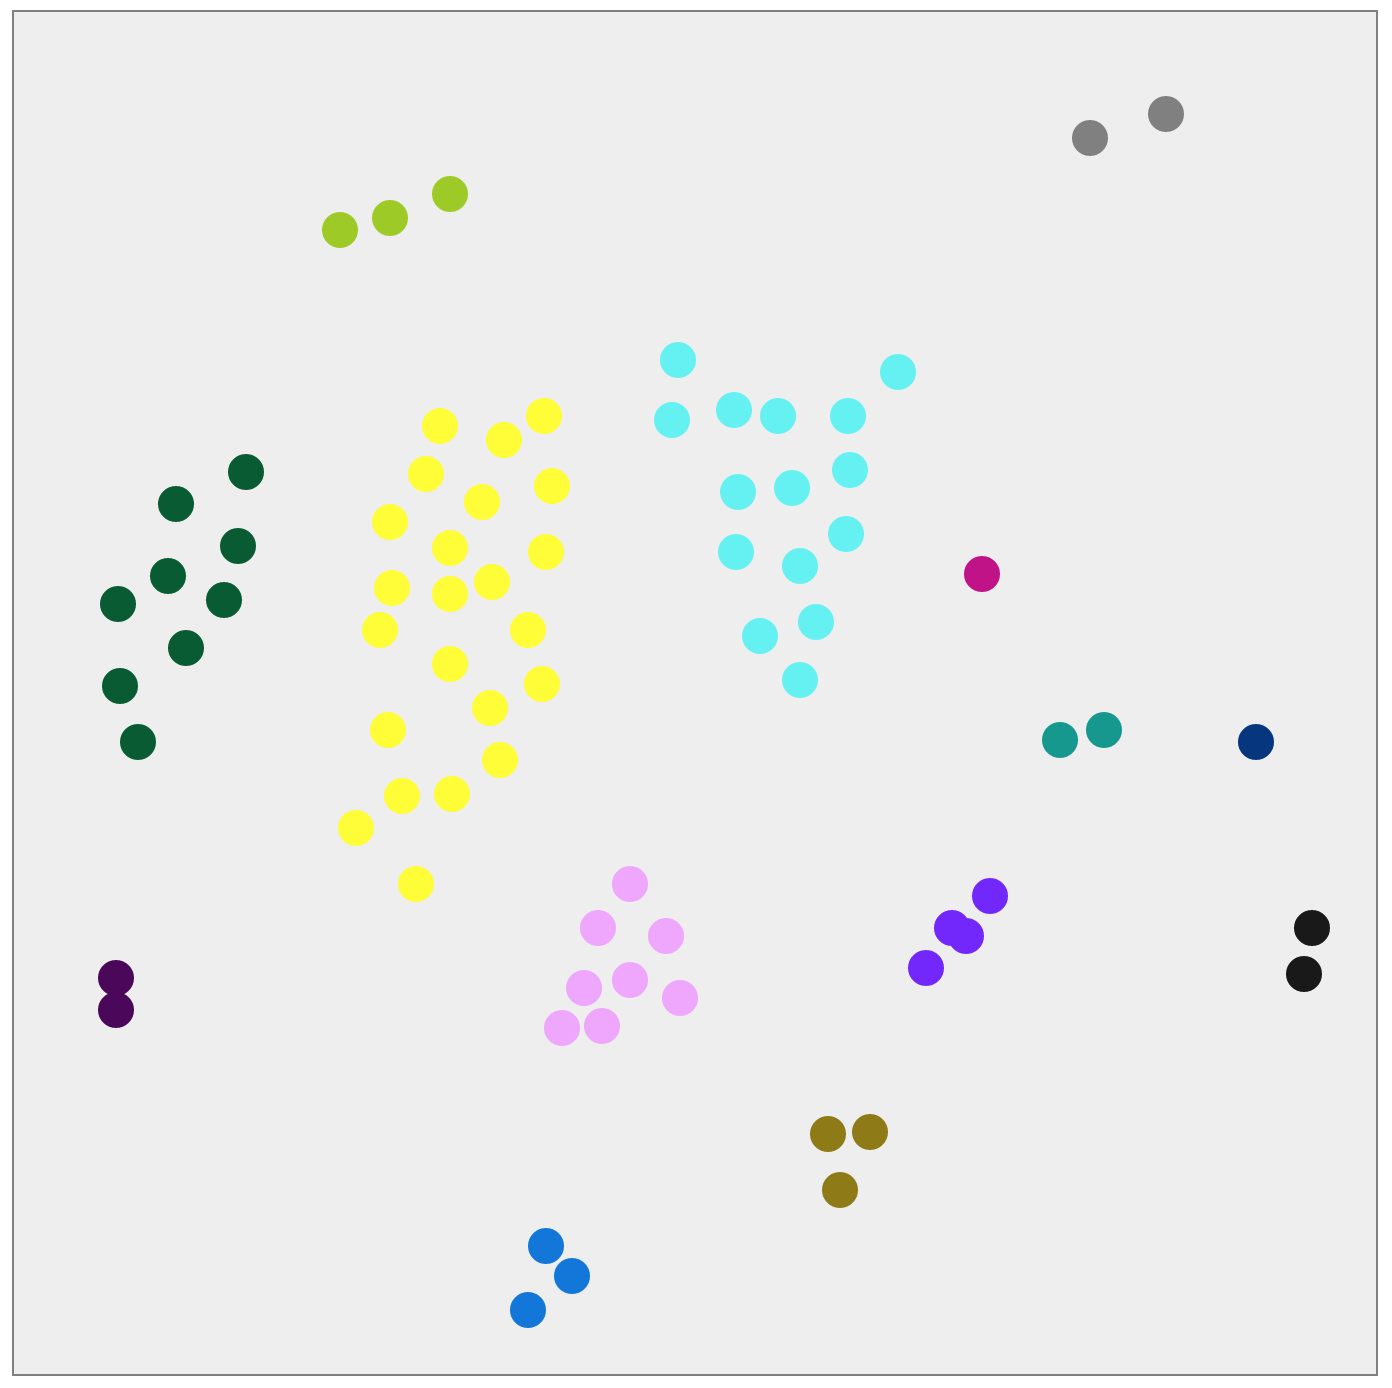
\includegraphics[width = \textwidth]{figures/xp2example.png}
\caption{Spatial and group organization provided by subject 1.}
\label{fig:xp2display}
\end{figure}

31 subjects completed the experiment. An example of resulting organisation of \ipt is given on Figure \ref{fig:xp2display}. The resulting organisation for each subject are available for reader's inspection using the full feature interface provided to the subjects for performing the experiment\footnote{https://mathieulagrange.github.io/paperSpontaneousSimilarity/demo}.

As discussed in the previous section, only the grouping given by the subjects using the color labels is considered to estimate the spontaneous judgments of similarity among \ipt. The spatial organisation of the dots representing the \ipt could provide information about the similarity, but this would implicitely force the fact that the timbral similarity space is two dimensional.

We therefore now only study the properties of the groupings performed by the subject prior to converting them into an overall similarity matrix.

Among the 20 colors available, the subjects used on average $10.2 \pm  4.1$ different colors to group \ipt. The distribution of the number of groups can be seen on Figure \ref{fig:xp2nbGroup}. The size of the groups is on average $7.7 \pm   7.2$. The distribution of the size of groups can be seen on Figure \ref{fig:xp2sizeGroup}. The large number of small groups indicates that many subjects considered that a few of the \ipt were very different from all the remaining \ipt.

\begin{figure}
\center
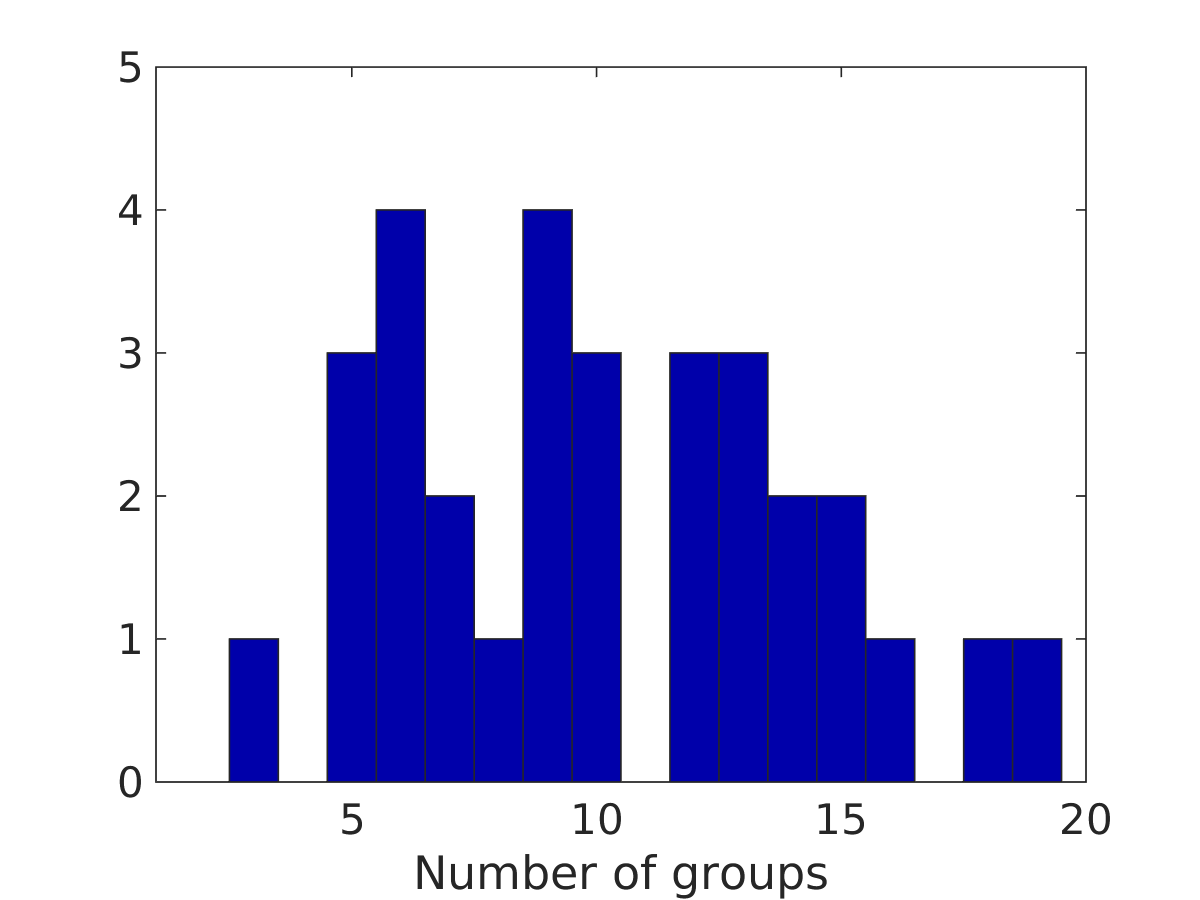
\includegraphics[width = \textwidth]{figures/nbc.png}
\caption{Histogram of the number of groups.}
\label{fig:xp2nbGroup}
\end{figure}

\begin{figure}
\center
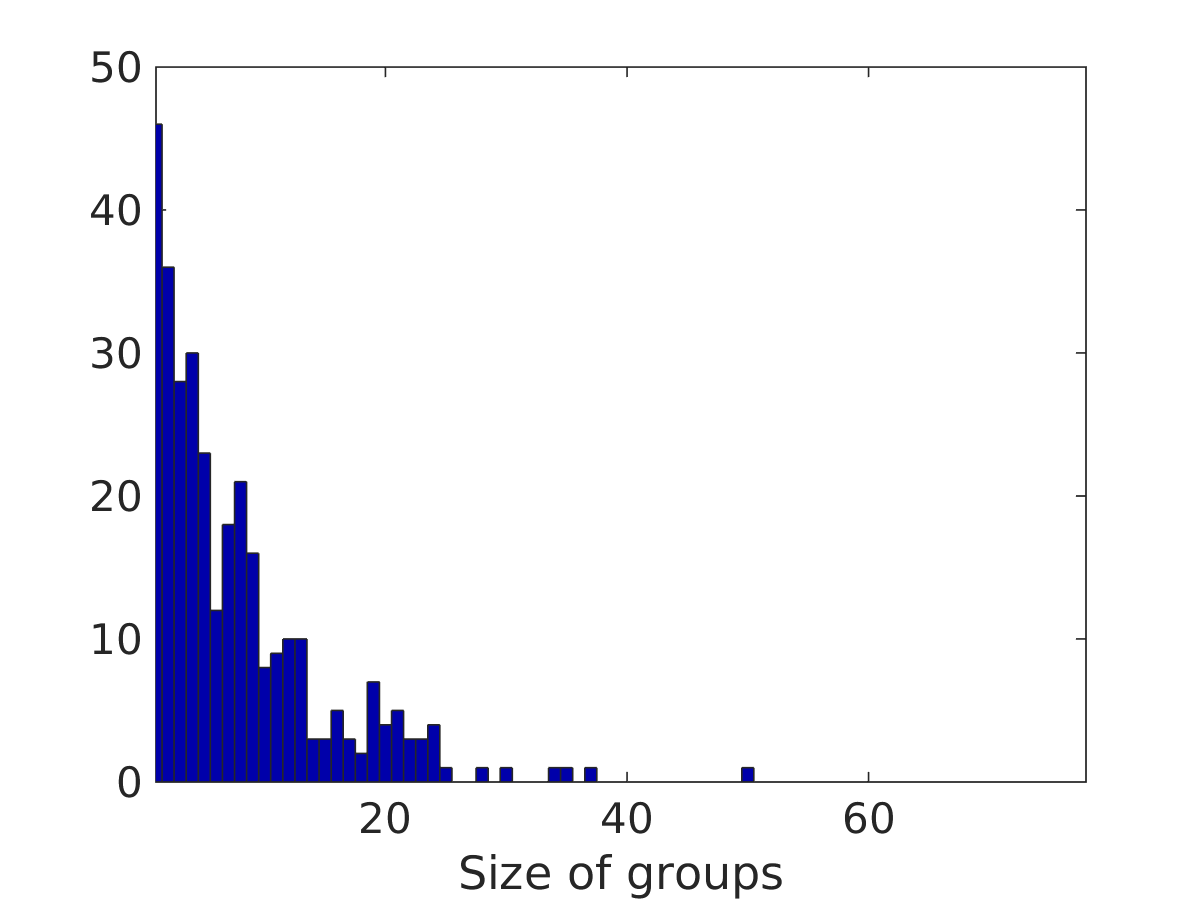
\includegraphics[width = \textwidth]{figures/sbc.png}
\caption{Histogram of the size of groups.}
\label{fig:xp2sizeGroup}
\end{figure}

A grouping can be considered as a binary similarity measure, with $s(a, b) = 1$ if $a$ and $b$ belong to the same group, and $0$ otherwise. By averaging the 31 binary similarity matrix, an overall floating point matrix is obtained that correponds to our measure of the spontaneous perceptual similarity between \ipt.

In order to gather information about the properties of the data, a cluster analysis is next performed using an agglomerative hierarchical clustering \cite{gordon1987review} using the weighted average algorithm for computing distance between clusters. The resulting dendrogram is displayed on Figure \ref{fig:dendrogram}. A partition of $n$ clusters can be constructed from the agglomerative hierarchical cluster tree by finding the smallest height at which a horizontal cut through the tree leaves $n$ clusters.

One question that arises is whether the similarity is influenced primarily by the instrument or by the playing technique. To answer this question, each partition provided by cutting the dendrogram at successive levels is compared to two reference partitions. One reference is the partition of the \ipt when labeled with the instrument used (I) and the other if the partition of the \ipt when labeled with the playing technique used (Pt).

There are many metrics to compare two partitions by evaluating their degree of correspondance \cite{wagner2007comparing}. The normalized mutual information (NMI) is interesting as it do not require alignement of the groups labels between the two partitions prior correspondance analysis and the two partition are not required to have the same number of groups. It also by design bounded between 0 and 1, 1 meaning perfect match. We consider the normalization proposed in \cite{strehl2002cluster}. Figure \ref{fig:clusters} shows the evolution of the NMI when comparing the partitions provided by the cluster analysis of the dendrogram produced using the human judgment of similarity and respectively the instrument partition ($j/I$) or the playing technique partition ($j/Pt$).

\begin{figure}
\center
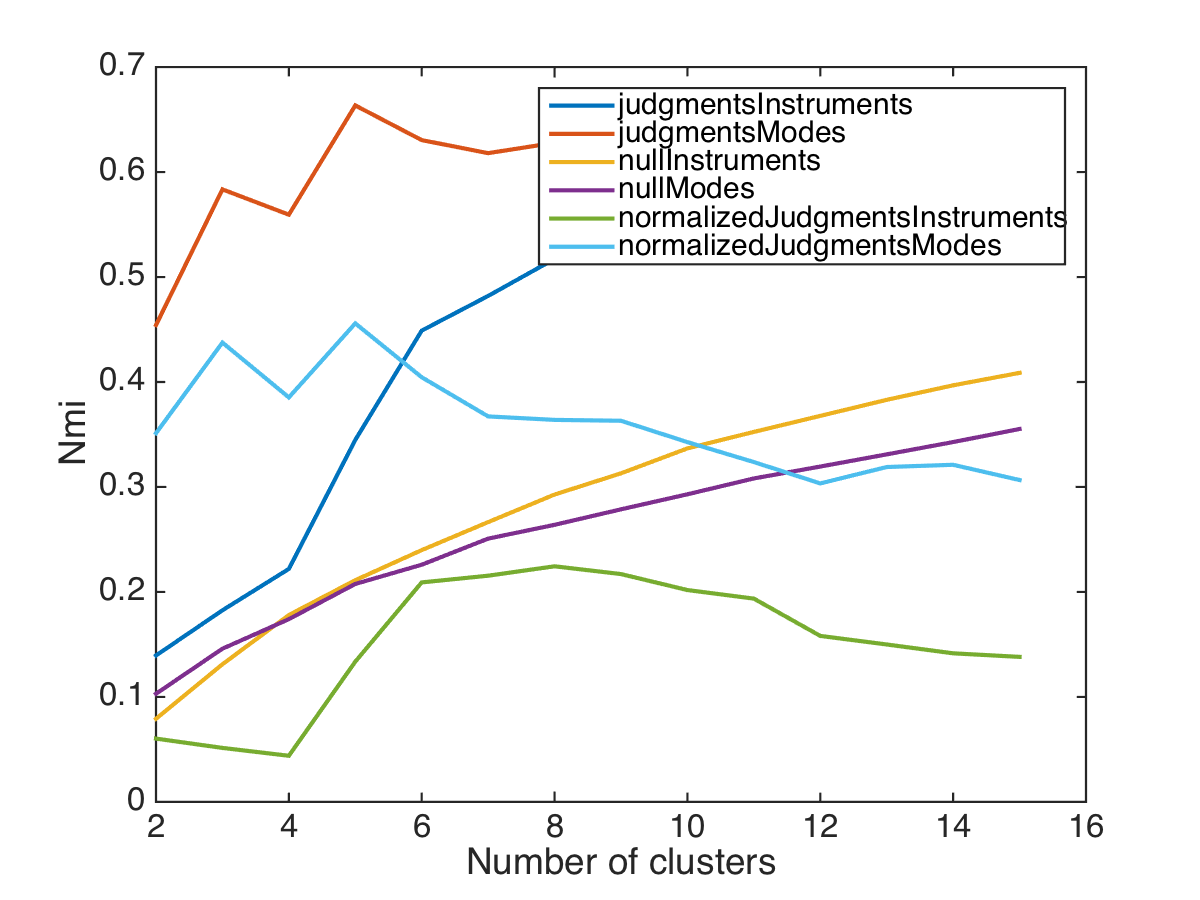
\includegraphics[width = \textwidth]{figures/clusterAnalysis.png}
\caption{Cluster analysis of the similarity judgments. $j/I$ and $j/Pt$ compare the partition obtained using the similarity judgments clustered using a growing number of clusters versus respectively the instrument partition and the playing technique partition. Normalizing factors $nullI$ and $nullPt$ are used to obtain normalized measures: $nj/I$ and $nj/Pt$. \ml{change legend}}
\label{fig:clusters}
\end{figure}

There is a clear gain of NMI when considering the playing technique which means that the subjects primarily used cues corresponding to the playing technique to organize the \ipt. Also, for both curves, a global trend of increase with respect to the number of clusters in the $j$ partition can be observed. This is a well documented fact, which simply put, means that it is easier to match any given partition with more clusters at hand \cite{tibshirani2001estimating}. To compensate for this bias, one can consider the NMI that would be achieved by comparing several random partitions of increasing number of clusters to the reference one, be it the instrument partition ($nullI$) or the playing technique partition ($nullPt$). The resulting averaged NMI for 100 randomly generated partitions are displayed on Figure \ref{fig:clusters}. Those curves are useful for normalizing $j/I$ and $j/Pt$ by simply substracting the so-called null NMIs:
\begin{eqnarray}
  nj/I &=& j/I - nullI  \\
  nj/Pt &=& j/Pt - nullPt  \\
\end{eqnarray}
This normalization is useful for identifying more easily the number of clusters for which the comparison is most relevant. As can be seen on Figure \ref{fig:clusters}, the number of clusters that leads to the highest NMI is 5 for the playing technique reference and 8 for the instrument reference, leading respectively to an NMI of $0.46$ and $0.21$. For the latter, reducing the number of clusters down to 6 do not decrease the NMI by much, a fact that will be latter discussed in more details. Even by considering the null normalization, the matching level is much higher for the playing technique reference.

The correspondances between those partitions and the reference ones are now studied. For this purpose, Figure \ref{fig:gi} displays two partitions. At the bottom is the partition that corresponds to the instruments labels, whose color code is given by the color bar on the right. The abbreviations used for the instruments are detailed in Section \ref{sec:dataset}. The ordering of \ipt on the horizontal axis is the one given by the cluster analysis, see the dendrogram on Figure \ref{fig:dendrogram}. The partition on top is the result of the clustering with 8 clusters. For visualization purposes, we arbitrarily set colors to clusters of this partition to the color code of the instrument label that is most often encountered in this cluster. If some labels occur equally often, the instrument of the first \ipt of the cluster is chosen. The emerging instrument classes are: Saxophone, Clarinet, Trumpet, Flute and Cello.

Though, even with an optimal number of clusters, we see that the clusters have  a low purity, \textit{i.e.} a very diverse set of instruments labels for the \ipt they belong to. Also, some clusters could be merged without stong changes in the overall organisation. This probably explains the small changes of NMI when reducing the number of clusters, see Figure \ref{fig:clusters}.

As can be seen on Figure \ref{fig:gm}, the correspondance between the playing technique reference and the resulting partition with 5 clusters is much higher. Most clusters have a high level of purity and for groups emerge : Pizzicato, Slap, Ordinario, and Ponticello.

To conclude this section, the process of gathering data about the perceptual similarity of \ipt is found to be successful as the subjects used their degree of freedom in a consistent manner and no inconsistency in the data has been detected during the analysis process. The main result is that the playing technique is an important factor when modeling the spontaneous judgment of similarity gathered in the second experiment.


\begin{figure}
\center
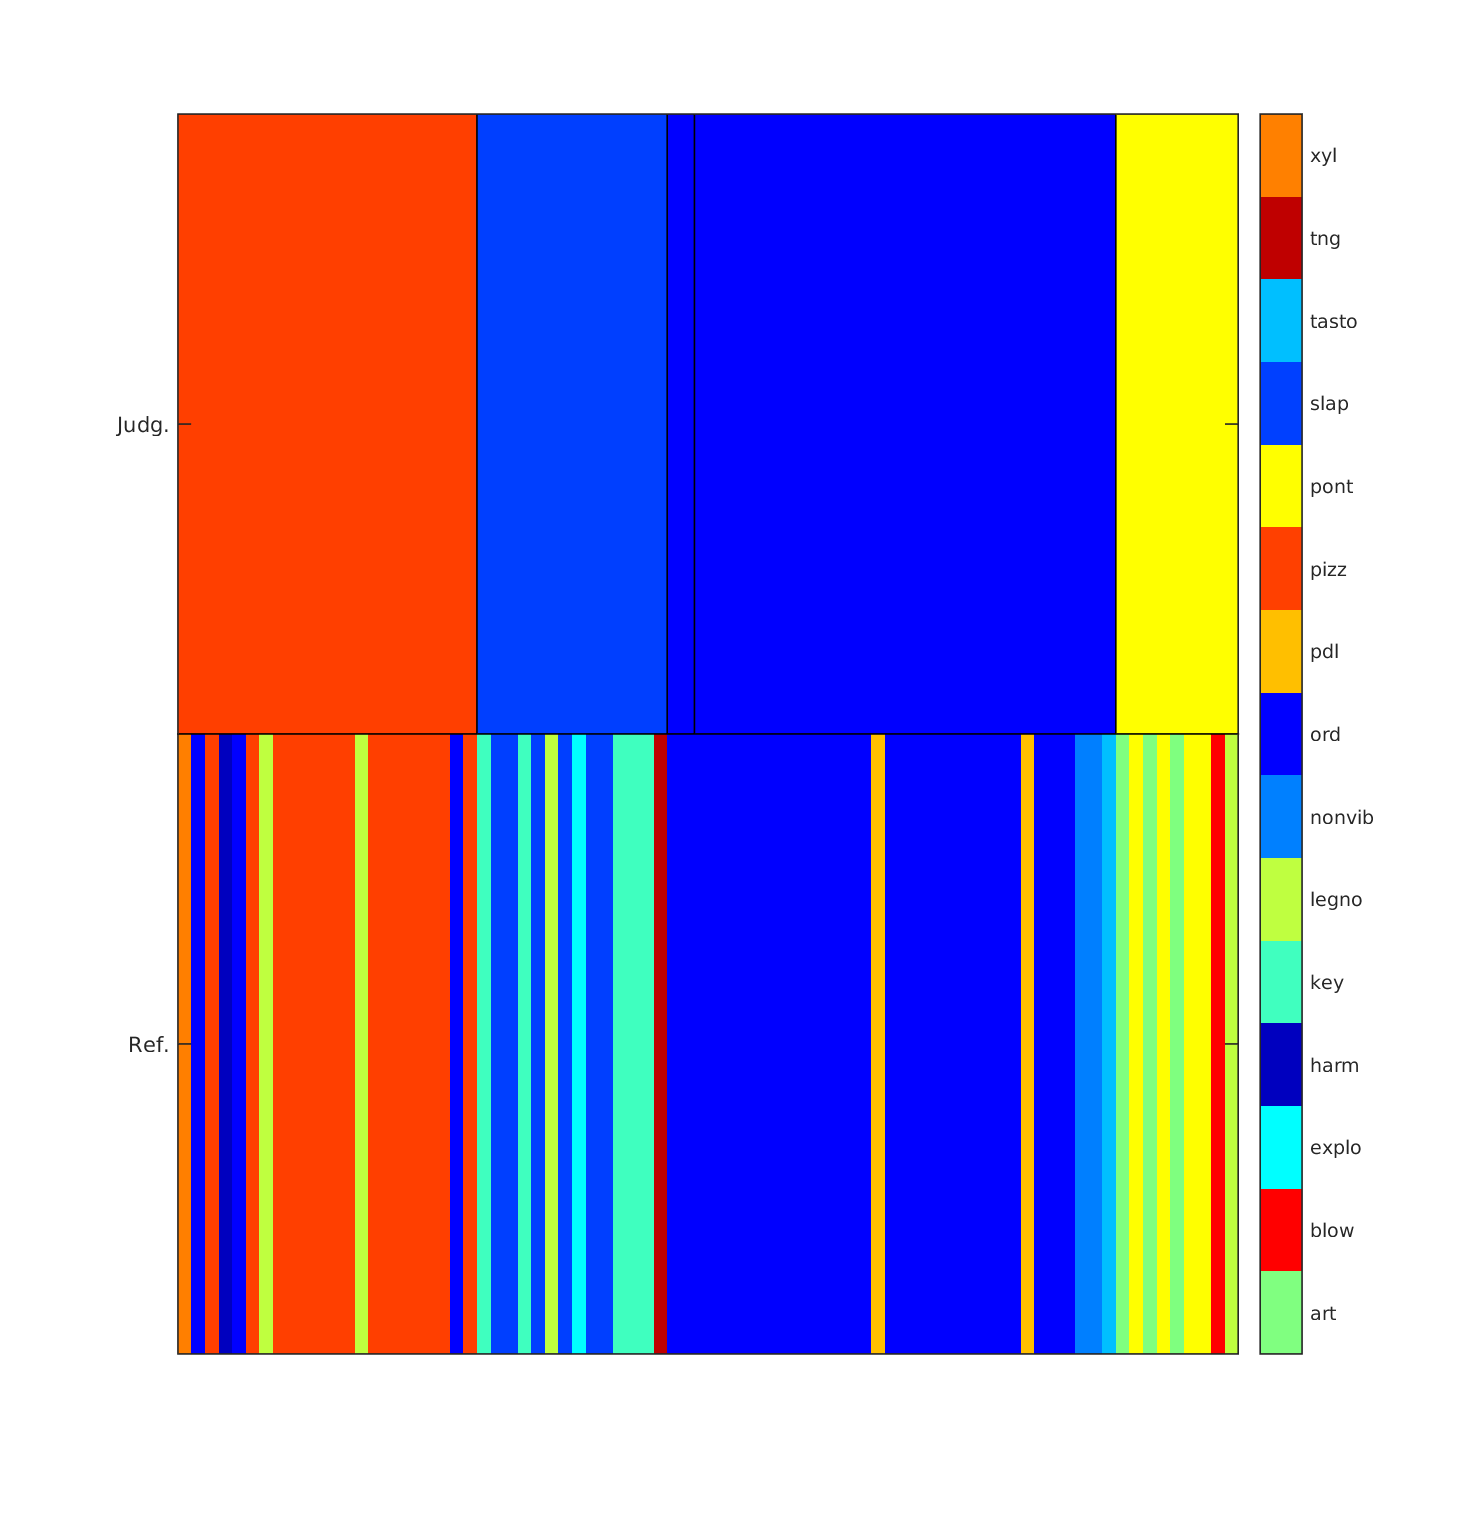
\includegraphics[width = \textwidth]{figures/groupModes.png}
\caption{Clustering \ipt using average perceptual similarity into 5 clusters (top) and playing technique labels (top). The color chosen to display each clusters on top corresponds to the playing technique that is dominant in this cluster, from left to right: 'pizzicato', 'slap', 'key', 'ordinario', 'ordinario', 'ponticello', 'art'.}
\label{fig:gm}
\end{figure}





\begin{figure}
\center
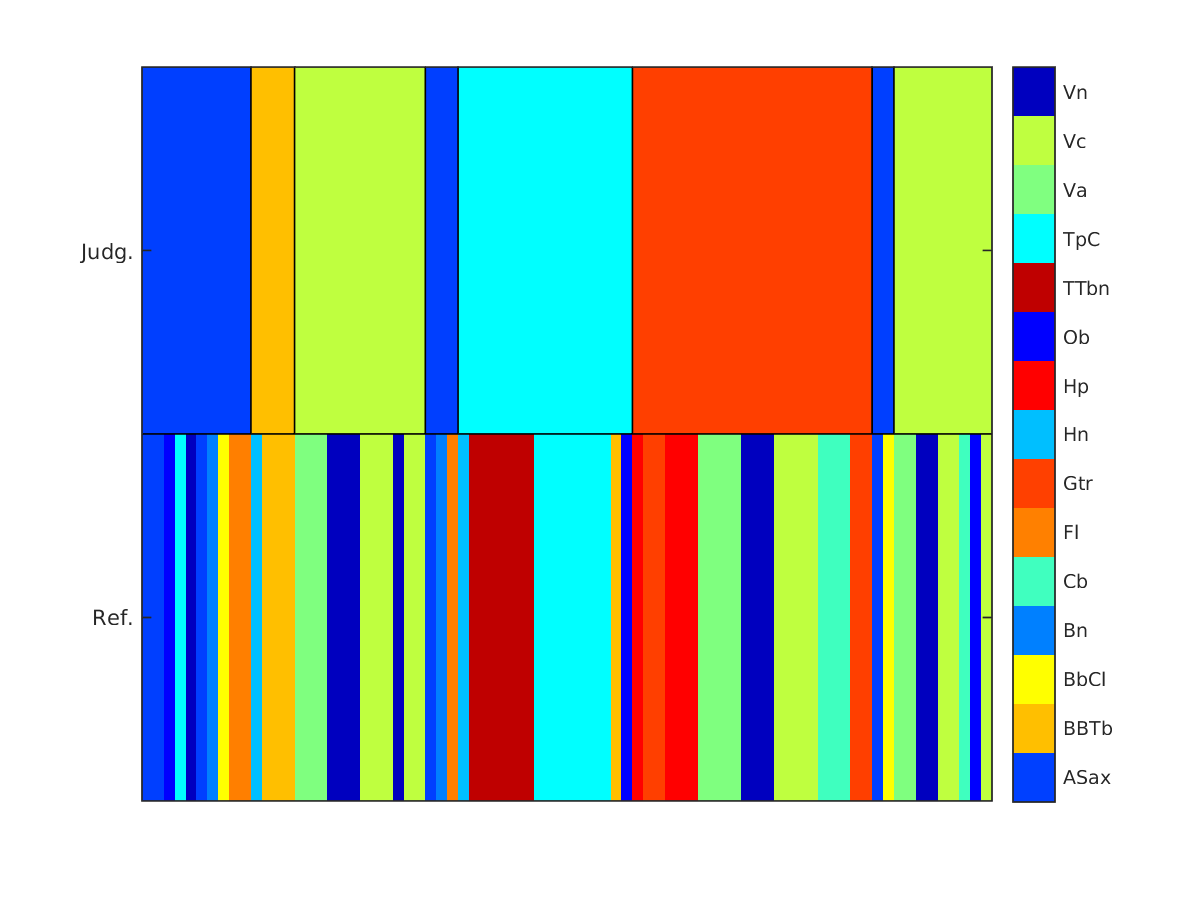
\includegraphics[width = \textwidth]{figures/groupInstruments.png}
\caption{Clustering \ipt using average perceptual similarity into 8 clusters (a) and instrument reference labels (b). The color chosen to display the groups (on top) corresponds  to the instrument that is dominant in this group, from left to right: 'ASax', 'BBTb', 'Vc', 'ASax', 'TpC', 'Gtr', 'ASax', 'Vc'.}
\label{fig:gi}
\end{figure}

\section{Model}\label{sec:model}

Once the perceptual data is gathered and controled, our aim is to evaluate the ability of the proposed perceptual model that is now introduced in more details. The model is composed of two processing stages, respectively called the primary and the secondary stage, see Figure \ref{fig:model}. The primary stage is designed to rely on very few meta parameters set arbitrarily by the experimenter to mimic the early stages of the mamalian auditory system. On contrary, the secondary stage rely largely on the data it has to model and in this respect mimic the high plasticity of the later stages of the mamalian auditory system.

\begin{figure}
\center
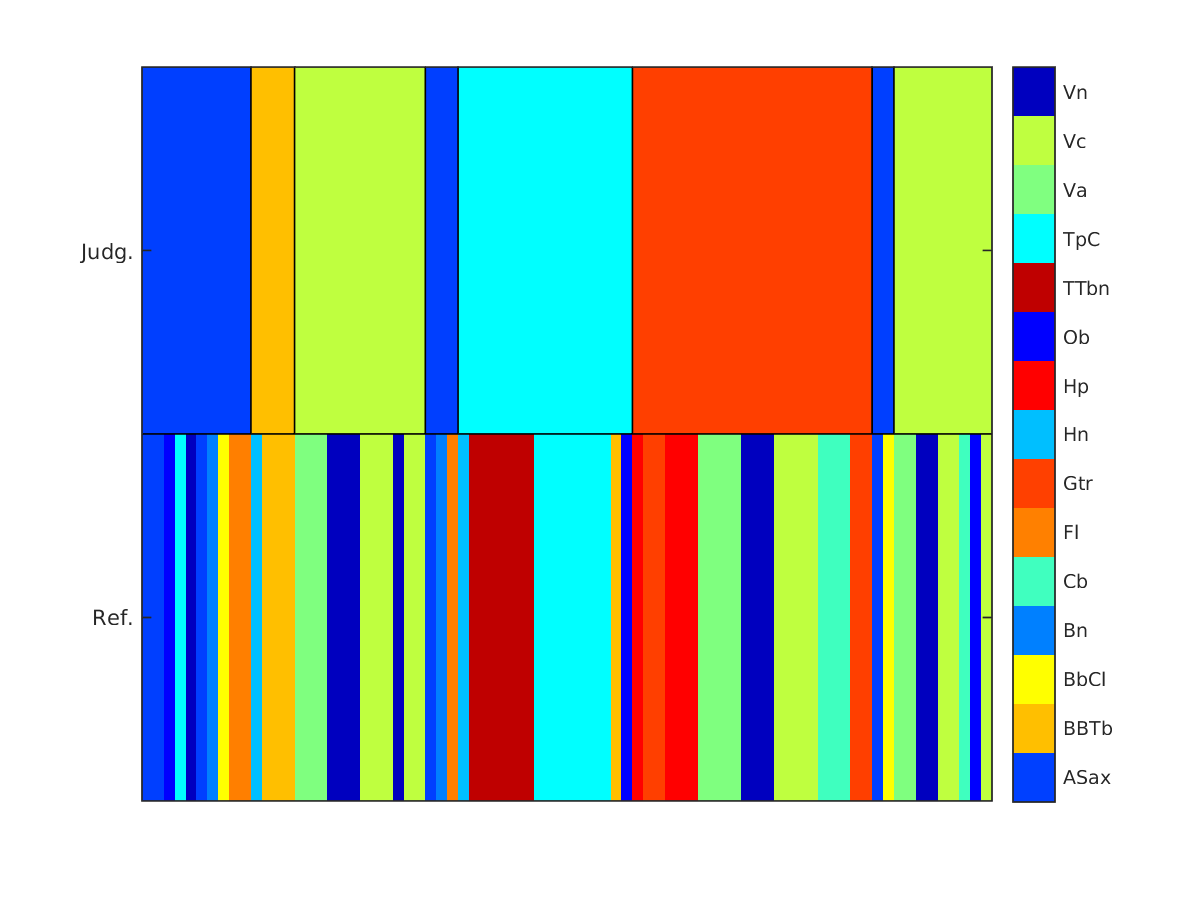
\includegraphics[width = \textwidth]{figures/groupInstruments.png}
\caption{Computational model \ml{TODO}}
\label{fig:model}
\end{figure}

\subsection{Primary stage}

In order to model the early stages of the mamalian auditory system, the time scattering transform \cite{anden2014deep}, obtained by applying a one dimensional
wavelet transform in time to a time-frequency wavelet scalogram. This transform thus encodes well modulations over time of energy distributed over frequency, dimensions that are shown to be perceptually important \cite{dau1997modeling}.

This model is chosen over more complex alternatives for the sake of simplicity. Deep convolutional networks could have been considered \cite{lee2009unsupervised}, but the learning stage inherent in this kind of methods did not seem relevant for this study. On contrary, the scattering transform can be conveniently parametrized to match the perceptual capabilities of the auditory system as those parameters are not expected to change significantly among subjects. Also, more complex versions of the scattering like the joint time-frequency scattering \cite{anden2015joint} and the spiral scattering \cite{lostanlen2016wavelet} are not considered in order to achieve a projection of reasonable dimensionality and for lack of evidence that those dimensions are mandatory to model the primary stage of the auditory system.

\subsection{Secondary stage}

The secondary stage involves a learning based process block that will weight the features outputed by the primary stage.

Indeed, if the properties of the first processing stages of the human auditory system can reasonably be considered as similar for every subjects despite potential hearing losses for some, the later ones is expected to vary more drastically due to their respective education, tastes and experiences with stimuli similar to the \ipt that are considered in this study. We therefore consider a supervised setting in order to optimize the representational space provided by the scattering transform. To do so, we will consider as our reference the clusterings provided by the subjects of experiment 2. Therefore, the goal of the secondary stage is to provide a metric space that closely match the one resulting from the data gathering by experiment 2.

To do so, one can first consider the linear discriminant analysis (LDA) \cite{duda2000pattern} to project the data into a representational space of $C-1$ dimensions with $C$ being the number of classes of the reference. The projection computed using this method is such that the ratio of the between-class distance
to the within-class distance is maximized, thus achieving maximum discrimination between elements of different class.

Another solution is to compute a projection matrix that maximizes the fact that neighbors in the representational space belong to the same class in the reference clustering while items from different classes are separated by a large margin. To do so, the large margin nearest neighbor (LMNN) metric learning algorithm \cite{weinberger2006distance, weinberger2009distance} is considered. One advantage of the latter is that the resulting representational space is of the same dimensionality as the input one whereas the LDA output dimentionality is contrained by the number of classes in the reference grouping.

Those methods are designed for considering only one reference grouping. Though, in our case, there is one reference grouping per subject. One approach is to find one consensus grouping that maximally represent the 31 reference groupings. In this paper, the chosen consensus grouping is taken from 3 solutions issued from 3 different algorithmic approach. This consensus is chosen as the one that has the best averaged NMI when compared to the 31 reference groupings \cite{strehl2002cluster}.

Another approach is to combine the projection matrices issued from the processing of the projection algorithm over the 31 reference groupings. As the number of classes can vary between reference groupings, the combination is not feasible using the LDA method. On contrary, the LMNN method can outputs a projection matrix per reference grouping. Those projection matrices being of the same dimensionality they can safely be averaged to estimate an consensus projection.



\section{Validation}\label{sec:validation}

As it will be discussed in the next Section, the main application scenario that is considered in this paper is the the recommandation of sounds based on examplar. This involves the definition of a similarity measure that behave similarly to the human perception, at least, that conform to the data we gathered in experiment 2.

Our problem is thus casted into a ranking problem, where from several candidates, the algorithm is asked to provide a ranking list of those candidates, sorted by similarity.

\subsection{Data}

As explained in the first section, gathering perceptual similarity data is plagued is plagued with a size problem. In order to provide enough data for the numerical analysis described in this section, we complement the data gathered during the second experiment as follows: for each \ipt, instead of one sound examplar we consider the whole range of nuance and pitch that is available. This leads to a dataset of 9346 sound recordings. It is thus assumed that the perceptual similarity is invariant with respect to pitch and nuance which is not necessarily true, but is taken here as a reasonable assumption.

\subsection{Metric}

The performance of the different methods are evaluated in a ranking setting. The precision at rank $k$ is thus considered, with $k=5$. For one sound recording termed the query, the $k$ the nearest other sound recordings are retrieved. The precision is then the ratio of those sound recordings that have the same label as the query in the grouping we consider as reference. This process is repeated for each sound recordings taken as query, and the performance is averaged over the queries.

\subsection{Methods}

To evaluate the performance of the proposed approach, several baselines are considered for comparison purposes. For the first stage, the well known Mel-Frequency Cepstral Coefficients (MFCC)s are considered \cite{rabiner1993fundamentals}. The MFCCs are computed from frame of 25ms, the number of mel bands is 40 and all the DCT coefficients are kept. The resulting features have a dimensionality of 40. The MFCCs are then standardized by removing the mean and dividing by the standard deviation computed over the dataset.

The time scattering is computed over a range frame sizes, from 25 ms to 1 second. The Q factor is set to 8 in order to obtain a frequency decomposition that is equivalent to the mel scale. As the frame increase, the dimensionality increases. The resulting scattering features are then logarithmically compressed and normalized using the median computed over the dataset.

The LDA method do not requires any setting of parameters and the LMNN method is set to optimize for a neigbors size of 5.

\subsection{Results}

For the sake of reproducibility, the code of the proposed method and the experimental protocol is available\footnote{https://github.com/mathieulagrange/paperSpontaneousSimilarity}. For convenience, the features (scattering and mfccs) are alos provided, but the software can be used to process from scratch the SOL database.

\section{Discussion}\label{sec:discussion}

Thanks to the digitization capabilities available, gathering large amount of audio recordings of \ipt is achievable and several databases are now available on the market. Browsing of such databases can be achieved by keyword based search. It requires that 1) the database is fully annotated with a precise ontology of instruments and playing techniques, 2) that the user has a precise understanding of this ontology, and 3) that the user a precise idea of the kind of timbre he is looking to find the \ipt he is searching for.

An interesting alternative type of search is the similarity content based search. Being solely based on sound, this kind of search can be used when querying by example. The user provides an example of the target sound to find \ipt that match the timbre description of the query, be it an onomatepea, a tone from another instrument or any kind of environmental sound.

The computational model proposed in this paper is well suited for this kind of search, as it can model complex perceptual timbre spaces and can scale to large databases. Once the features and the projection matrix are computed, the similarity computation is quite effective and can be further enhanced by considering fast similarity search scheme such as locally sensitive least square hashing \cite{pauleve2010locality}. The secondary stage being learnt, it can easily adapt to user tastes and usage history by reweighting the scattering features for improved search relevance.

\bibliographystyle{alpha}
\bibliography{bib}

\section{Dataset} \label{sec:dataset}

The dataset considered in this paper as been recorded at Ircam and is composed of audio recording of 16 different musical instruments played with different playing techniques, which leads to 143 different couple of instrument / playing technique. For each couple, the pitch and intonation is varied leading to 25444 audio samples.

The recorded instruments belongs to the wind and string classes. For winds, the instruments considered in the second experiment are: accordion (Acc), saxophone alto (ASax), tuba (Tb), bassoon (Bn), clarinet Bb (BbCl), flute (Fl), horn (Hn), oboe (Ob), trombone tenor (TTbn), and trumpet C (TpC). For the string class, the instruments are: guitar (Gtr), harp (Hp), viola (Va), violin (Vn), violoncello (Vc), and contrabass (Cb).

Some instruments can be complemented with sordina (S), wha (W). The addition of this kind of device modifying the shape of the instrument, a saxophone alto and saxophone alto with sordina are considered as different instruments.

Those instruments are recorded for different nuance and pitch if the latter is relevant, but more importantly, several playing technique are considered. For  the second experiment described in this paper, the playing techniques considered are: artificial harmonic (art), blow (blow), exploding slap  (explo), harmonic (harm), key-click (key), col legno   (legno), non vibrato (nonvib), ordinario (ord), pedal tone (pdl), pizzicato (pizz), ponticello (pont), slap (slap), (tasto), tongue-ram (tng), and xylophonic (xyl).

\section{Dendrogram}


\begin{figure}
\center
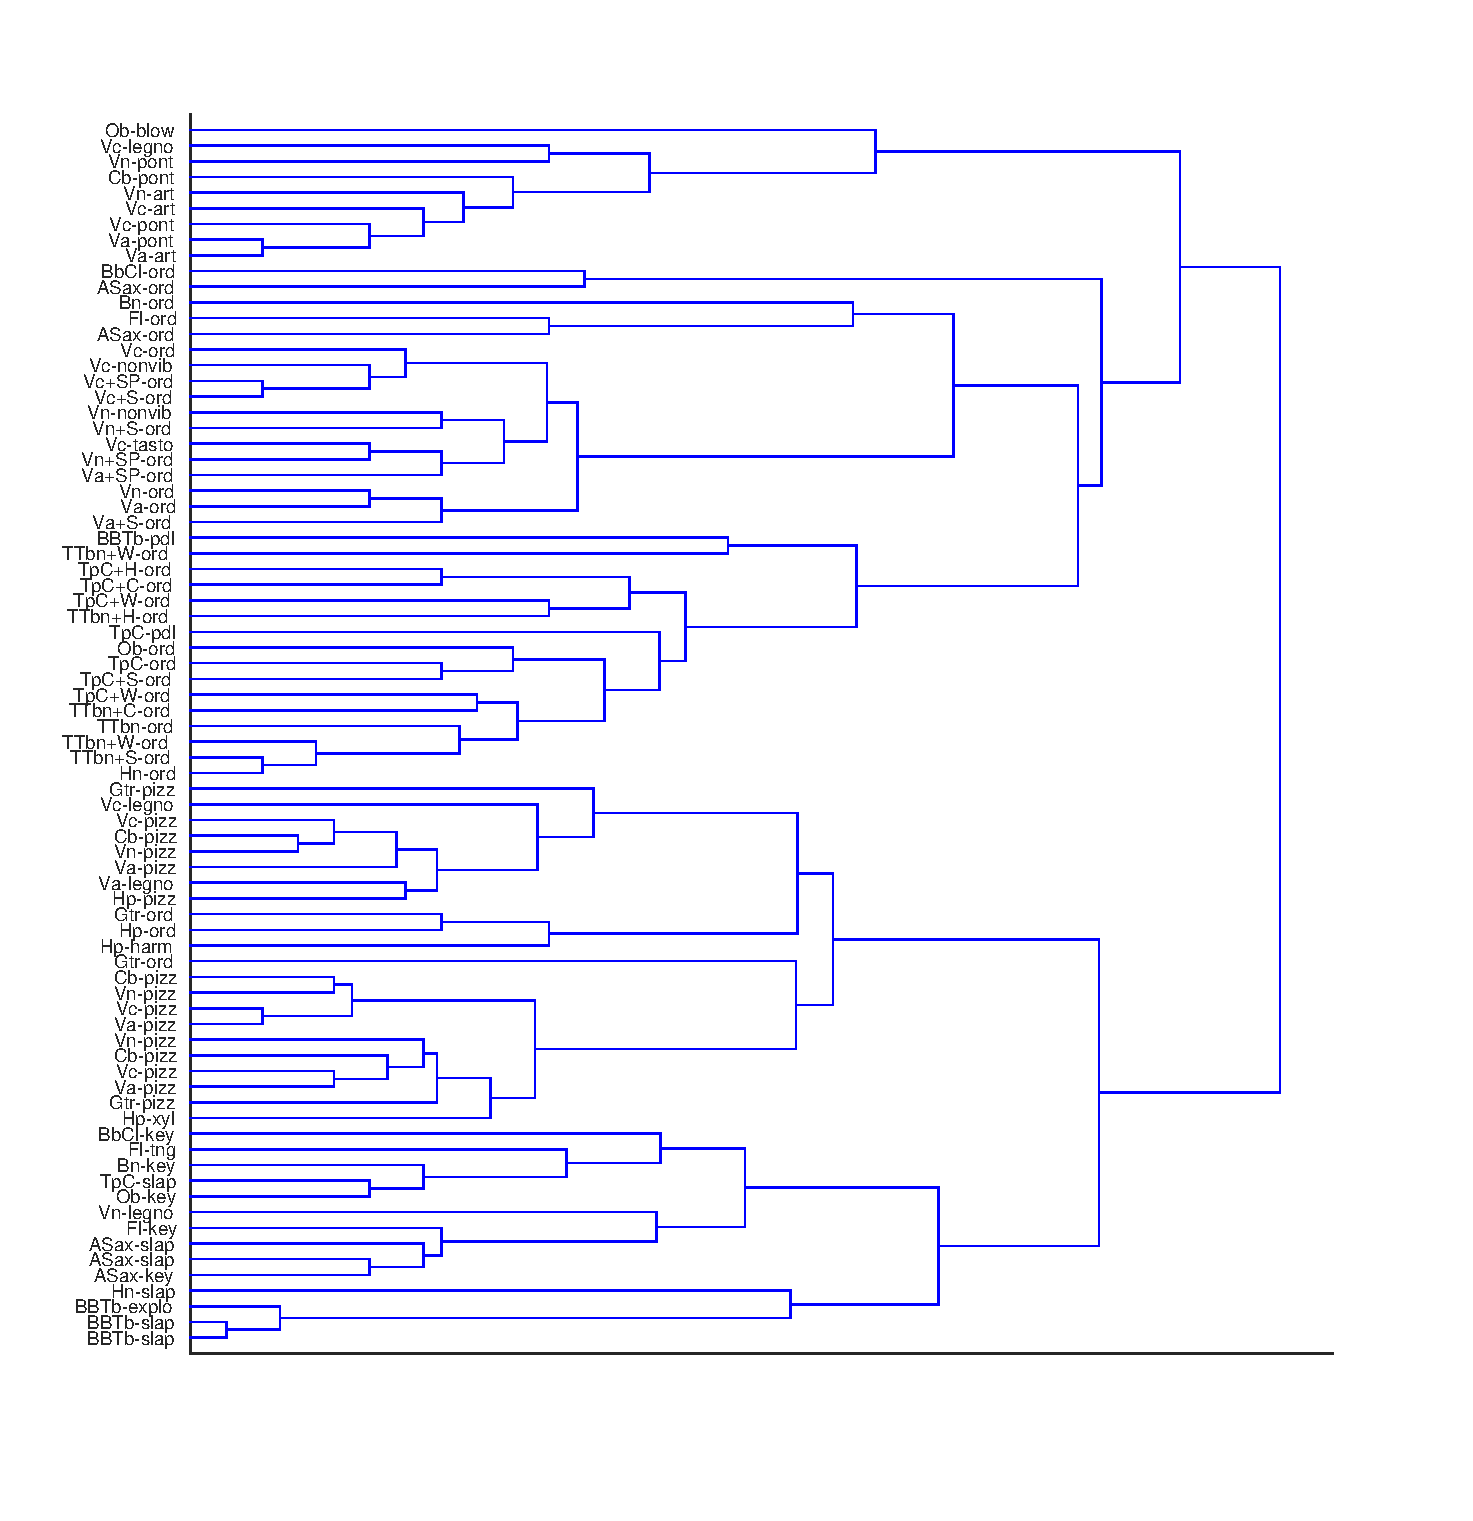
\includegraphics[width = \textwidth]{figures/dendrogram.pdf}
\caption{Dendrogram obtained after processing the similarity judgment matrix using the agglomerative clustering algorithm.}
\label{fig:dendrogram}
\end{figure}

\end{document}
